\documentclass[12pt]{article}
\usepackage[margin=1in]{geometry}
\usepackage{setspace}
\onehalfspacing

% Start of preamble
%==========================================================================================%
% Required to support mathematical unicode
\usepackage[warnunknown, fasterrors, mathletters]{ucs}
\usepackage[utf8x]{inputenc}

\usepackage[dvipsnames,table,xcdraw]{xcolor}

% Standard mathematical typesetting packages
\usepackage{amsmath,amssymb,amscd,amsthm,amsxtra, pxfonts}
\usepackage{mathtools,mathrsfs,dsfont,xparse}

% Symbol and utility packages
\usepackage{cancel, textcomp}
\usepackage[mathscr]{euscript}
\usepackage[nointegrals]{wasysym}
\usepackage{apacite}

% Extras
\usepackage{physics}  
\usepackage{tikz-cd} 
\usepackage{microtype}
\usepackage{enumitem}
\usepackage{titling}
\usepackage{graphicx}

% Fancy theorems due to @intuitively on discord
\usepackage{mdframed}
\newmdtheoremenv[
backgroundcolor=NavyBlue!30,
linewidth=2pt,
linecolor=NavyBlue,
topline=false,
bottomline=false,
rightline=false,
innertopmargin=10pt,
innerbottommargin=10pt,
innerrightmargin=10pt,
innerleftmargin=10pt,
skipabove=\baselineskip,
skipbelow=\baselineskip
]{mytheorem}{Theorem}

\newenvironment{theorem}{\begin{mytheorem}}{\end{mytheorem}}

\newtheorem{corollary}{Corollary}
\newtheorem{lemma}{Lemma}

\newtheoremstyle{definitionstyle}
{\topsep}%
{\topsep}%
{}%
{}%
{\bfseries}%
{.}%
{.5em}%
{}%
\theoremstyle{definitionstyle}
\newmdtheoremenv[
backgroundcolor=Violet!30,
linewidth=2pt,
linecolor=Violet,
topline=false,
bottomline=false,
rightline=false,
innertopmargin=10pt,
innerbottommargin=10pt,
innerrightmargin=10pt,
innerleftmargin=10pt,
skipabove=\baselineskip,
skipbelow=\baselineskip,
]{mydef}{Definition}
\newenvironment{definition}{\begin{mydef}}{\end{mydef}}

\newtheorem*{remark}{Remark}

\newtheorem*{example}{Example}

% Common shortcuts
\def\mbb#1{\mathbb{#1}}
\def\mfk#1{\mathfrak{#1}}

\def\bN{\mbb{N}}
\def \C{\mbb{C}}
\def \R{\mbb{R}}
\def\bQ{\mbb{Q}}
\def\bZ{\mbb{Z}}
\def \cph{\varphi}
\renewcommand{\th}{\theta}
\def \ve{\varepsilon}
\newcommand{\mg}[1]{\| #1 \|}

% Often helpful macros
\newcommand{\floor}[1]{\left\lfloor#1\right\rfloor}
\newcommand{\ceil}[1]{\left\lceil#1\right\rceil}
\renewcommand{\qed}{\hfill\qedsymbol}
\renewcommand{\P}{\mathbb P\qty}
\newcommand{\E}{\mathbb{E}\qty}
\newcommand{\Cov}{\mathrm{Cov}\qty}
\newcommand{\Var}{\mathrm{Var}\qty}

% Sets
\usepackage{braket}

\graphicspath{{/}}
\usepackage{float}

\newcommand{\SET}[1]{\Set{\mskip-\medmuskip #1 \mskip-\medmuskip}}

% End of preamble
%==========================================================================================%

% Start of commands specific to this file
%==========================================================================================%

%==========================================================================================%
% End of commands specific to this file

\title{CSE Template}
\date{\today}
\author{Rohan Mukherjee}

\begin{document}
    \maketitle
    \begin{enumerate}[leftmargin=\labelsep]
        \item \begin{enumerate}[label=(\alph*)]
            \item For a bunch of different values of $n$ and $\sigma$, LS usually returns something around $\pm 0.02$, and PCA returns something around $\pm 1$. For true independence, you would expect $E((X-E(X))(Y-E(Y))) = 0$, and as that is what LS returns, that is what you would get normally. On the other hand, if we write our data matrix $Z = \begin{pmatrix}
                x & y
            \end{pmatrix}$, then $Z^TZ = \begin{pmatrix}
                x^Tx & x^Ty \\
                x^Ty & y^Ty
            \end{pmatrix}$, and since $x^Tx, y^Ty \approx \sigma^2$, while $x^Ty \approx 0$, we get the eigenvectors of this matrix that PCA returns is just: $\begin{pmatrix}
                1 \\ 1
            \end{pmatrix}$ and $\begin{pmatrix}
                1 \\ -1
            \end{pmatrix}$. Since they have the same eigenvalue, PCA might return either of them, so we should get $\pm 1$. However, I am not fully sure why it chooses these eigenvectors instead of the standard basis ones, I think its probably an artifact of how the algorithm is initialized (presumably, you would only have to do one iteration of the power method).

            \item Here is the picture of that or only $y$ noise:
            \begin{figure}[H]
                \centering
                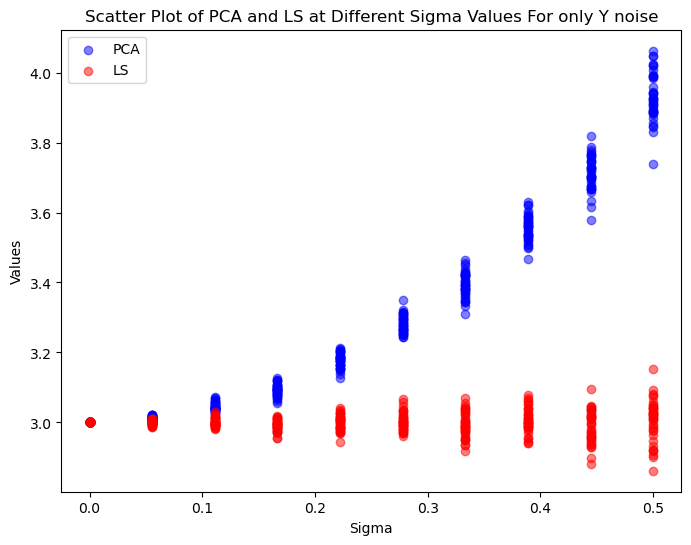
\includegraphics[width=0.5\textwidth]{y_noise.png}
            \end{figure}

            \item This is the scatter plot I got for both $x$ and $y$ noise:
            \begin{figure}[H]
                \centering
                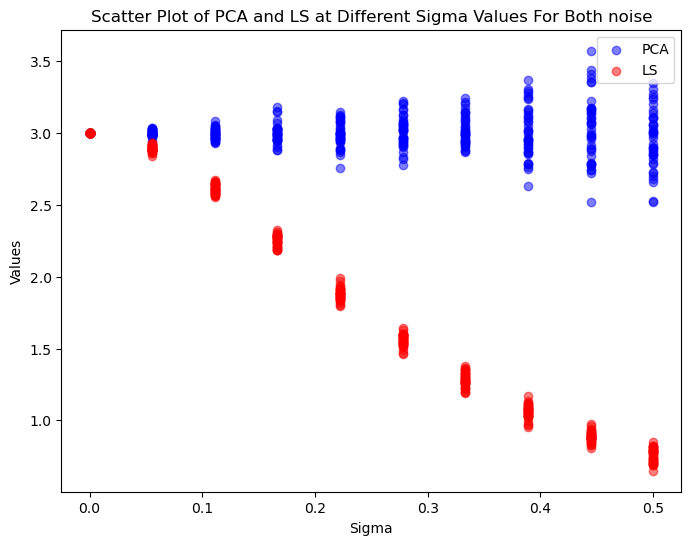
\includegraphics[width=0.5\textwidth]{x_y_noise.png}
            \end{figure}

            \item From the matrix before, if $y = 3x$, we should $Z^TZ = \mg{x}^2\begin{pmatrix}
                1 & 3 \\
                3 & 9
            \end{pmatrix}$ which (after removing the $\mg{x}^2$), has largest eigenvalue of 10 with corresponding eigenvector $\begin{pmatrix}
                1 \\ 3
            \end{pmatrix}$. However, if there is noise on only the $y$, with $y = 3x = \ve$ where $\ve \sim N(0, \sigma^2 I_n)$, then $x^Tx$, stays the same while $x^Ty = x^T(y + \ve) = x^Ty + x^T\ve = 3x^Tx + x^T\ve$, where $x^T \ve $is a $N(0, \sum x_i^2 \sigma^2)$ random variable. For large $\sigma$, this should be $3x^Tx$ but in reality can be very different from it, and the last coordinate $y^Ty = 9x^Tx + 6x^T \ve + \ve^T\ve$ also has giant variance. So the direction of PCA can be very spread out, which is what we observe for large $\sigma$.

            However, if there is noise on both the $x$ and $y$, recall that PCA is trying to find the direcdtion of maximum variance. Since we are making the noise in both $x$ and $y$ independently with same variance, the noise in the $x$ direction and $y$ direction equals proportionally. So, from the matrix, we would get something like: $\begin{pmatrix}
                x^Tx + 2x^T \ve_x + \ve_x^T\ve_x & 3x^Tx + x^T \ve_x \\ 
                3x^Tx + x^T \ve_y & 9x^Tx + 6x^T\ve_y + \ve_y^T\ve_y
            \end{pmatrix}$
            The second order error terms become small, and now as we have equal spread in the $x$ and $y$ directions, PCA will be robust and return the correct eigenvalue of $3$. Before, we only have spread in the $y$ direction which confused the PCA.

            For noise on both $x$ and $y$, we are outputting for LS: $(x + \ve_x - \mu_x \mathbf{1})^T(3x + \ve_y - \mu_y\mathbf{1}) / \mg{x + \ve_x - \mu_x\mathbf{1}}$, since the mean of $\ve_x$ and $\ve_y$ are both 0. 
            This gives has an error term of $\ve_x^T (3x) + x^T \ve_y$, which has a giant variance, being normally distributed with mean 0 and variance $\sigma^2 \sum_i (4x_i)^2$. This is like $4 \cdot 333$ times $\sigma^2$ in variance. So LS gets very confused and is super susceptible to noise, which gets crushed in this case. The error term $\ve_x^T(3x)$ is dominant, and was not present before where LS worked well. It causes a lot of variance which didn't happen before.
        \end{enumerate}
        \item \begin{enumerate}[label=(\alph*)]
            \item Here is the plot of the first 2 PCs:
            \begin{figure}[H]
                \centering
                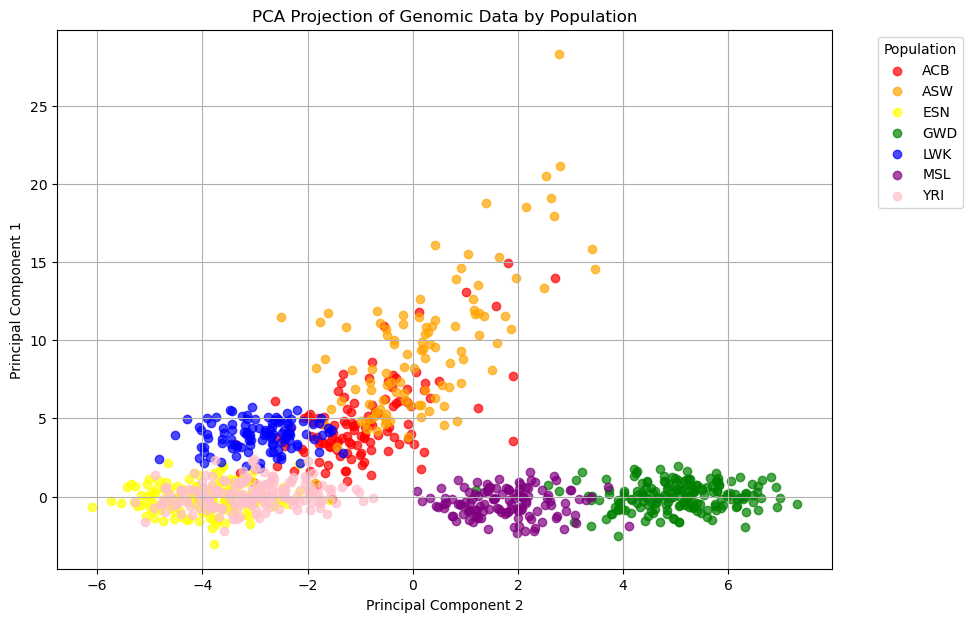
\includegraphics[width=0.5\textwidth]{2_pcs.png}
            \end{figure}
            \item MSL and GWD, being Mende, Sierra Leone and Gambian, Western Division, Mandinka are extremely close geographically, while still being on the African continent. ESN and YRI, being Yoruba in Ibadan, Nigera, and Esan in Nigera, are also clearly both in Nigeria, which explains why they are close in the PCA. Nigeria is very far east from Sierra Leone and Gambia, which explains the distinct spread between the two groups. The blue group, being noticeably above ESN and YRI can be explained since it means kenya, which is far to the east of Nigeria. It is extremely far from the green and purple group because of the large geographical gap between west and east Africa.
            The orange and red group, being ACB and ASW, are African Caribbeans in Barbados and Americans of African ancestry are both located in the Americas, namely closer to North America, extremely far away from Africa. This is why there is such a big spread between them and everything else. So it seems that the second PC represents the east/west divide in Africa, and the first represents the America/Africa geographical divide.

            \item Here is the plot of the first vs 3rd PCs:
            \begin{figure}[H]
                \centering
                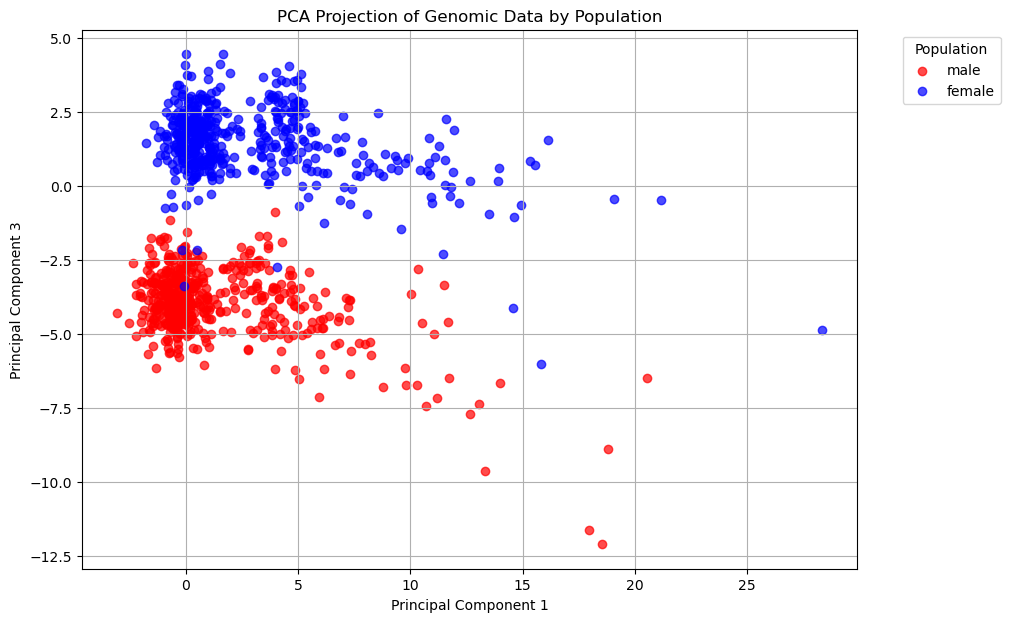
\includegraphics[width=0.5\textwidth]{1_3_pcs.png}
            \end{figure}

            \item I mean this is as clear as day. The third PC is repesentative of if the sample was a man or a woman.

            \item Let $x \in \R^n$ be a vector to be chosen later, and $X \in \R^{m \times n}$ be our data matrix, and consider
            \begin{align*}
                \tilde{X} = \begin{pmatrix}
                    X \\ x^T
                \end{pmatrix}
            \end{align*}
            Then,
            \begin{align*}
                \tilde{X}^T \tilde{X} = \begin{pmatrix}
                    X^T & x
                \end{pmatrix}\begin{pmatrix}
                    X \\ x^T
                \end{pmatrix} = X^TX + xx^T
            \end{align*}
            Using eigendecomposition of $X^TX$, which is the right singular vectors, we get $X^TX = \sum_i \sigma_i^2 v_iv_i^T$. We have been given that the first 3 are unique. If we now strategically choose $x = \sqrt{\sigma_1^2 - \sigma_2^2} v_2$, we can see that $v_1v_1^T$ and $v_2v_2^T$ now have the same coefficients and hence the first principal component is no longer unique.

            Similarly, if the first $k+1$ are unique, we can choose $x = \sqrt{\sigma_k^2 - \sigma_{k+1}^2}v_{k+1}$ and make the $k$th PC not unique.
        \end{enumerate}
    \end{enumerate}
\end{document}